\section{Spatio-temporal Class Activation Mapping}
\label{appendix:st-cam}

We describe the spatio-temporal class activation mapping (ST-CAM) which is extended from spatial CAM of the original paper~\cite{zhou2016CAM}.
We use a SlowOnly-50 ($8\times8$) network~\cite{feichtenhofer2019slowfast} which is pretrained on Kinetics-400~\cite{kinetics} dataset. 

To obtain a ST-CAM of a given video input, we first extract the final feature map of the SlowOnly-50 network before the global average pooling layer. 
The temporal dimension of the feature map is $8$ which is the same as the number of input frames.
We reduce the spatial stride of the last convolution from $2$ to $1$ of the original SlowOnly-50 network, so that the spatial dimension of the feature map is $14 \times 14$ to clearly see the CAM heatmap, while the original size is $7 \times 7$.
The number of channels of the feature map is $2048$.
Then, similar to the original paper~\cite{zhou2016CAM}, the extracted final feature map $(2048\times8\times14\times14)$ is multiplied with the fully-connected layer's weight corresponding to the target class $(2048\times1)$, resulting in $(8\times14\times14)$-dimensional spatio-temporal class activation mapping.
We sub-sampled $4$ frames of the ST-CAM in the main paper due to the limit of page width. 

We present additional ST-CAM visualizations in Figure~\ref{supp:cam1},~\ref{supp:cam2},~\ref{supp:cam3}, and~\ref{supp:cam4} which show the VideoMix samples and corresponding class activation maps with respect to the two action classes. 


\begin{figure*}[!t]
\centering
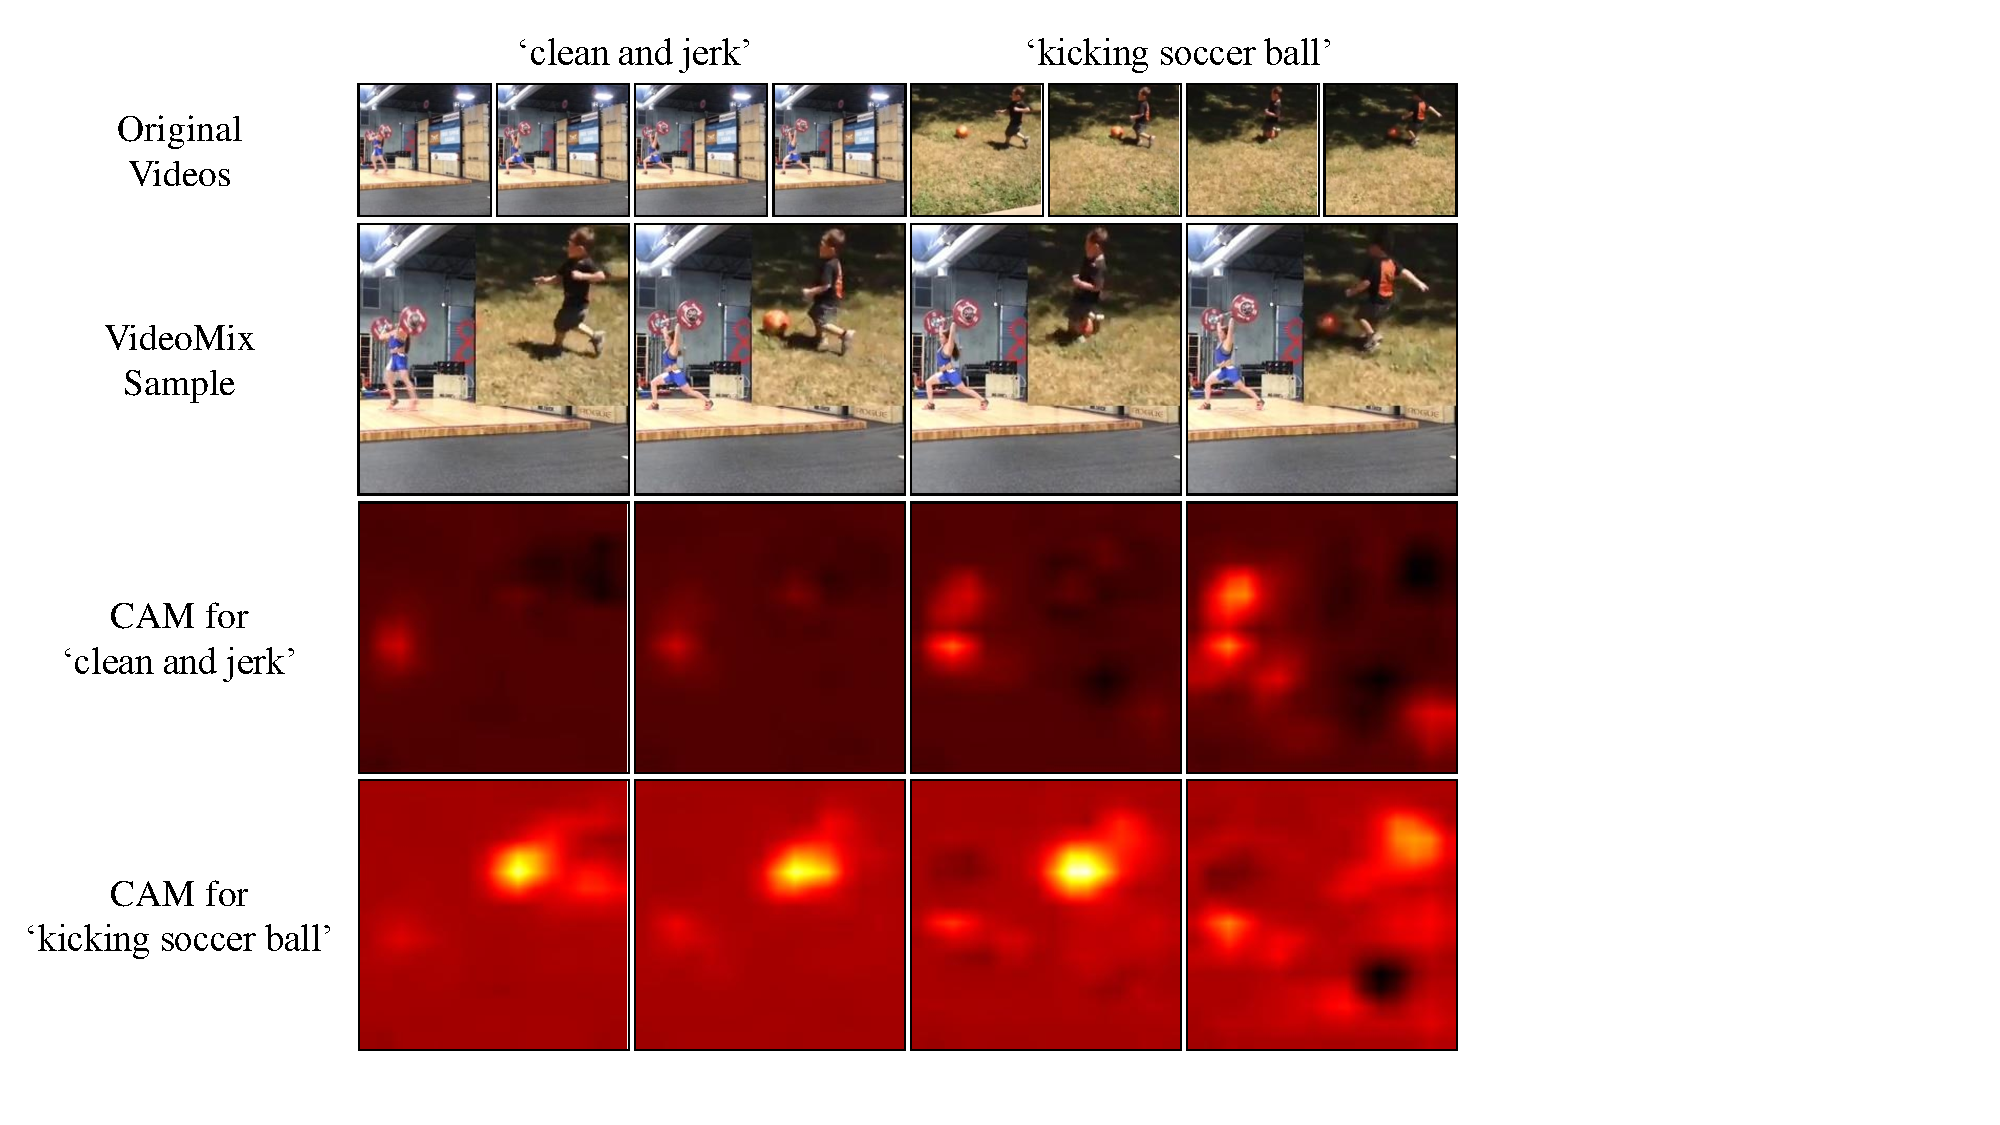
\includegraphics[width=0.77\linewidth]{arxiv_videomix/supplementary/figs/cam_supp1.pdf}
\caption{Spatio-temporal class activation mapping (ST-CAM) on VideoMix sample of the ``clean and jerk'' and ``kicking soccer ball'' videos.}
\label{supp:cam1}
\end{figure*}
\begin{figure*}[!t]
\centering
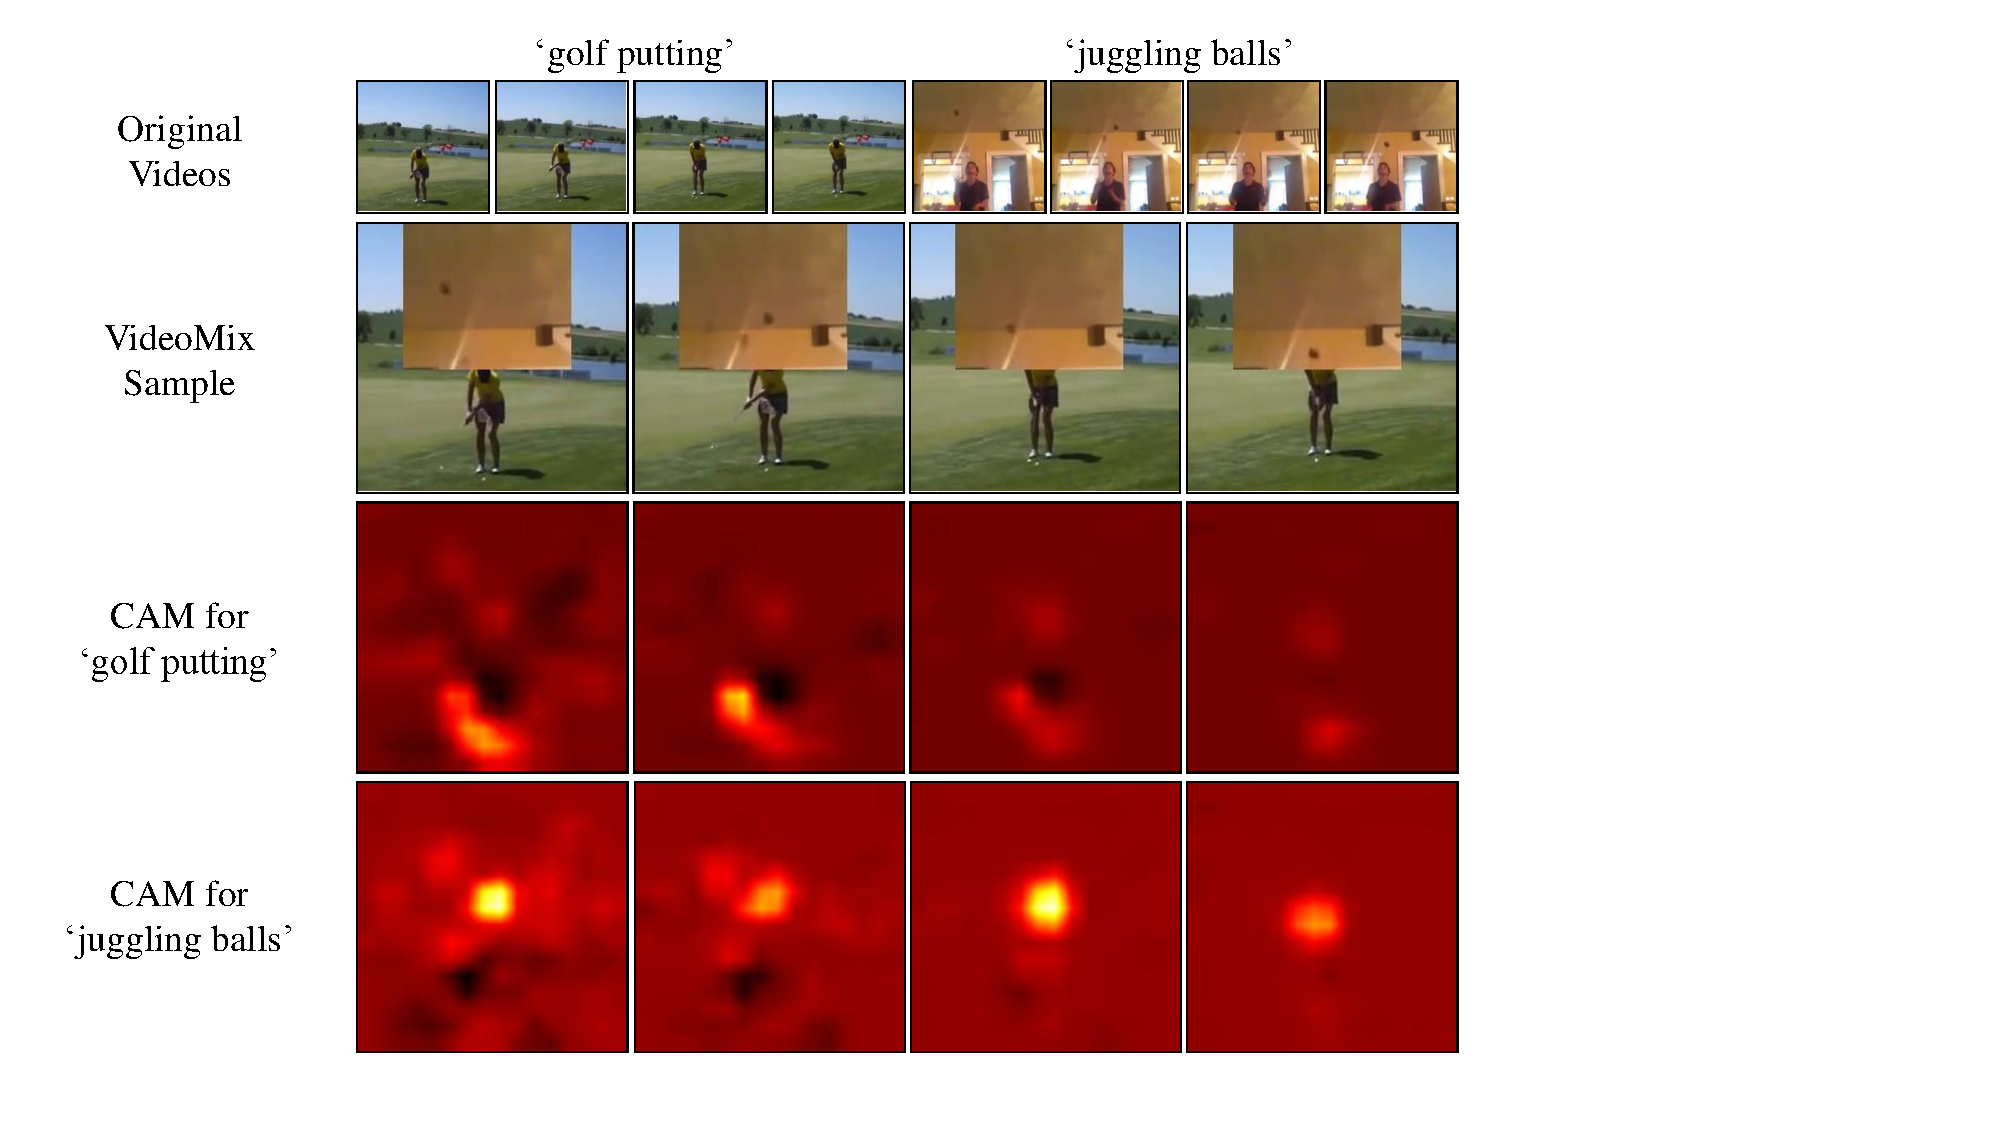
\includegraphics[width=0.77\linewidth]{arxiv_videomix/supplementary/figs/cam_supp2.pdf}
\caption{Spatio-temporal class activation mapping (ST-CAM) on VideoMix sample of the ``golf putting'' and ``juggling balls'' videos.}
\label{supp:cam2}
\end{figure*}
\begin{figure*}[!t]
\centering
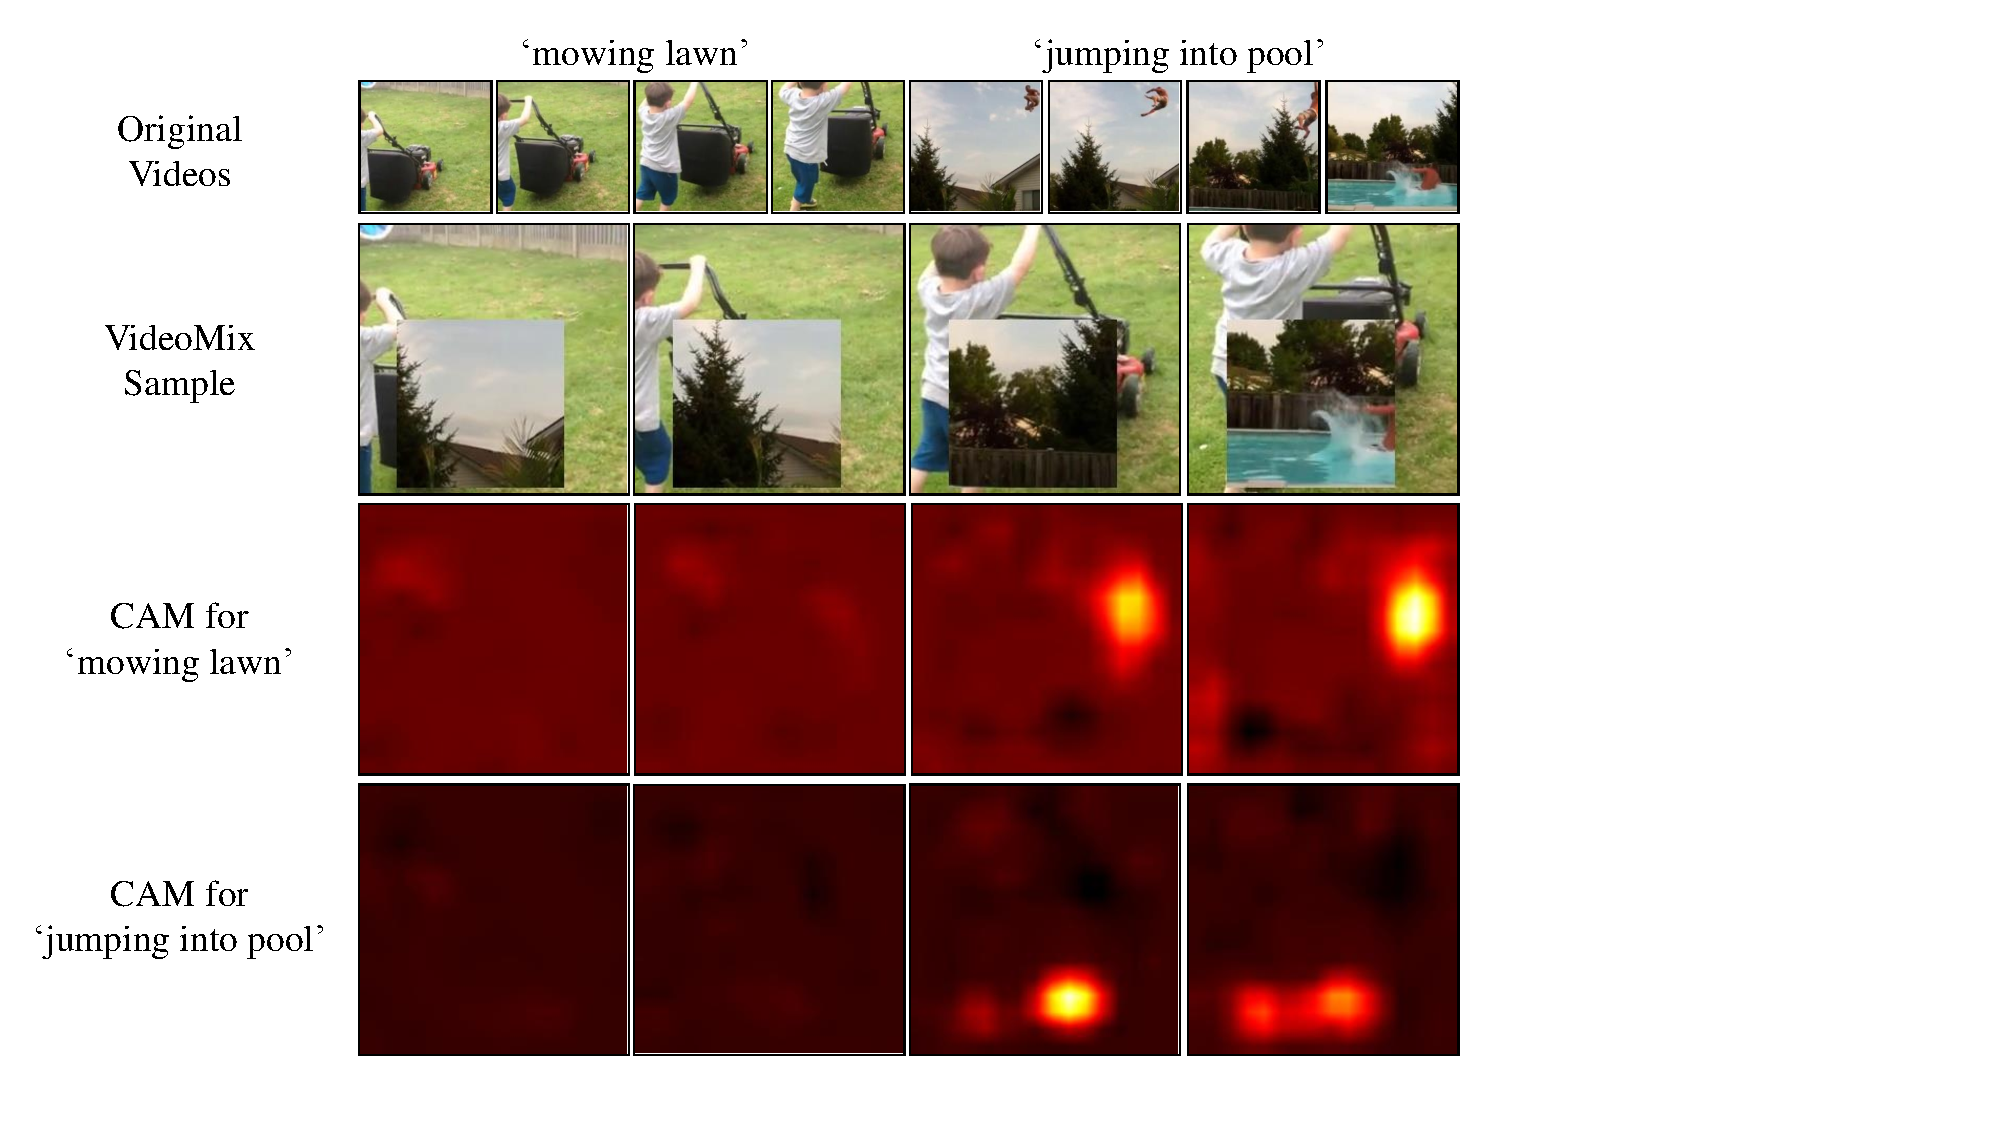
\includegraphics[width=0.77\linewidth]{arxiv_videomix/supplementary/figs/cam_supp3.pdf}
\caption{Spatio-temporal class activation mapping (ST-CAM) on VideoMix sample of the ``mowing lawn'' and ``jumping into pool'' videos.}
\label{supp:cam3}
\end{figure*}
\begin{figure*}[!t]
\centering
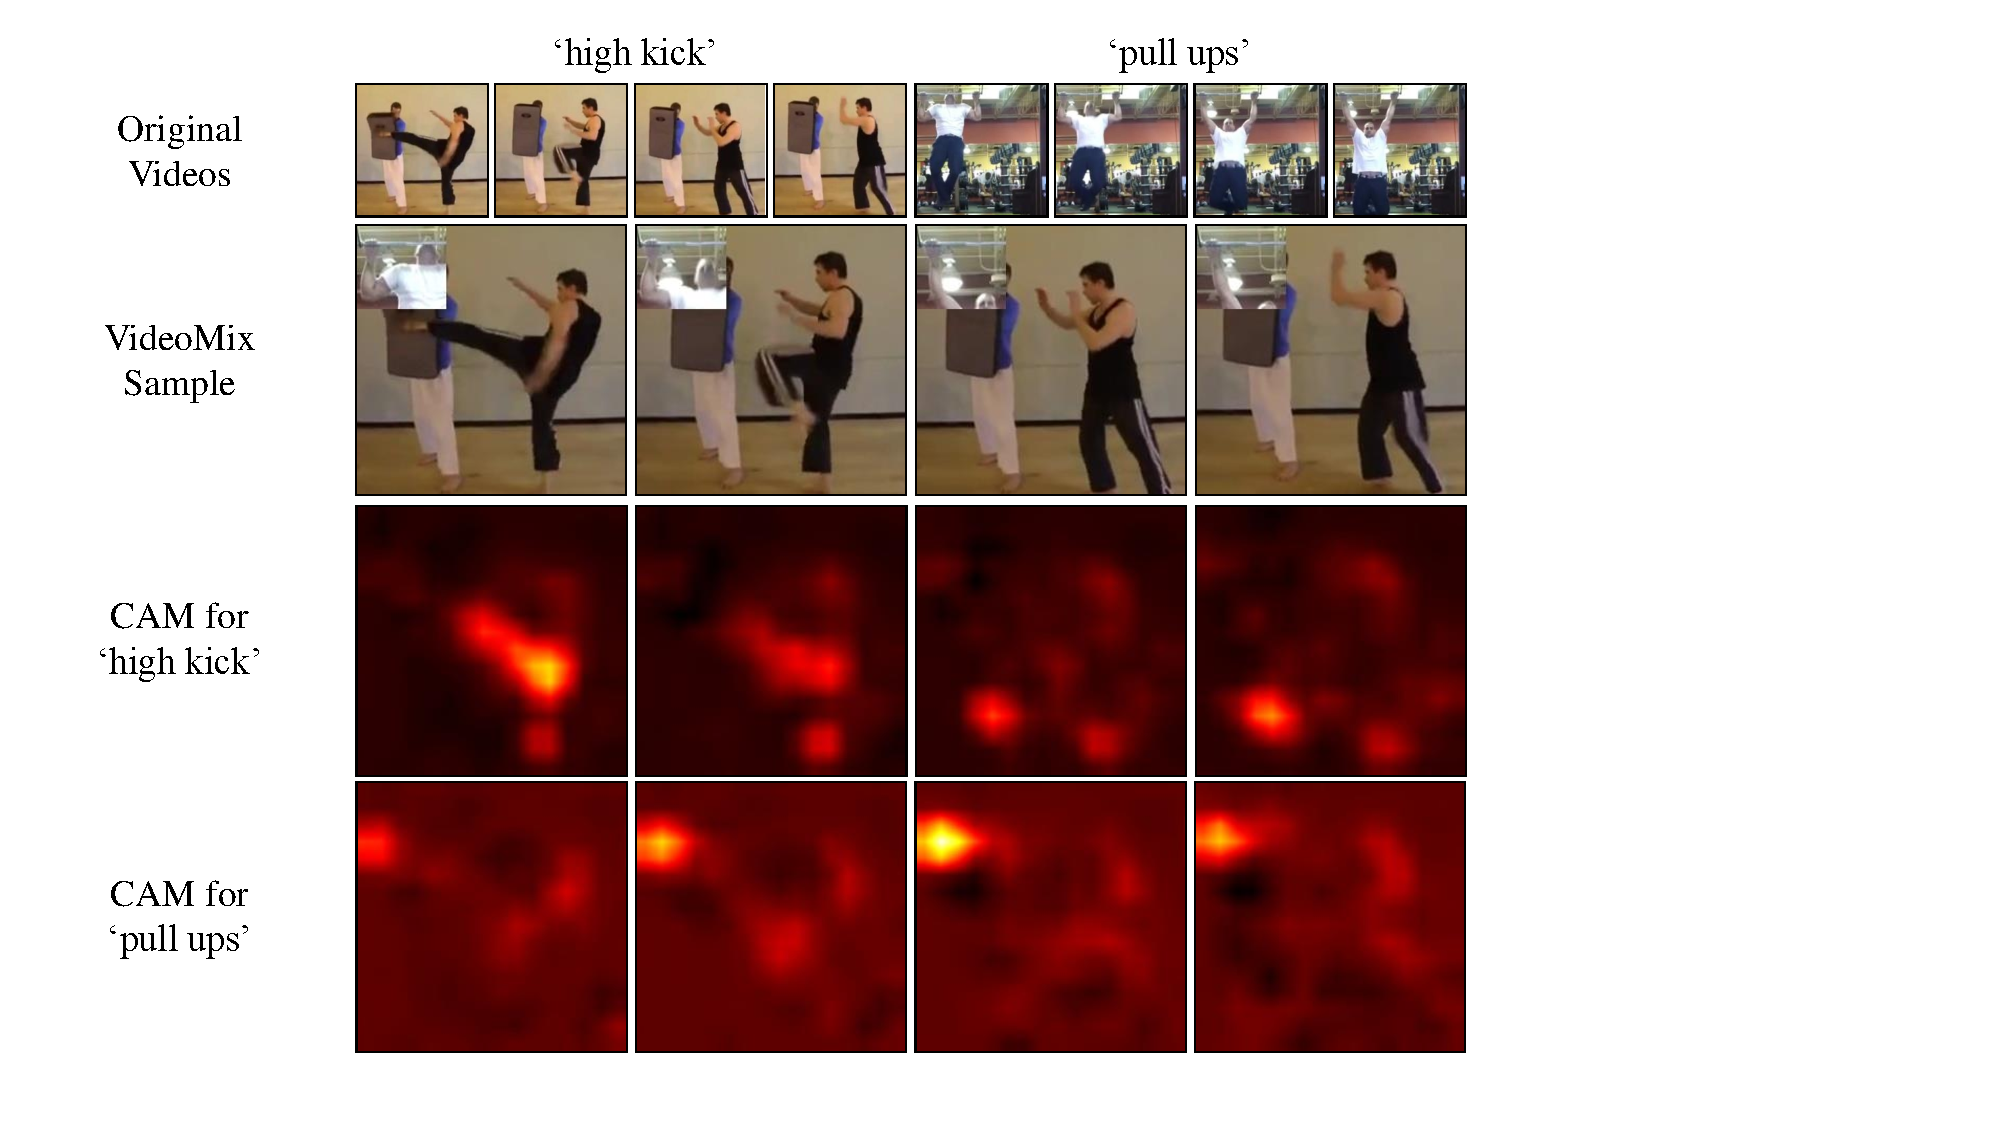
\includegraphics[width=0.77\linewidth]{arxiv_videomix/supplementary/figs/cam_supp4.pdf}
\caption{Spatio-temporal class activation mapping (ST-CAM) on VideoMix sample of the ``high kick'' and ``pull ups'' videos.}
\label{supp:cam4}
\end{figure*}
